\documentclass[]{tufte-handout}

% ams
\usepackage{amssymb,amsmath}

\usepackage{ifxetex,ifluatex}
\usepackage{fixltx2e} % provides \textsubscript
\ifnum 0\ifxetex 1\fi\ifluatex 1\fi=0 % if pdftex
  \usepackage[T1]{fontenc}
  \usepackage[utf8]{inputenc}
\else % if luatex or xelatex
  \makeatletter
  \@ifpackageloaded{fontspec}{}{\usepackage{fontspec}}
  \makeatother
  \defaultfontfeatures{Ligatures=TeX,Scale=MatchLowercase}
  \makeatletter
  \@ifpackageloaded{soul}{
     \renewcommand\allcapsspacing[1]{{\addfontfeature{LetterSpace=15}#1}}
     \renewcommand\smallcapsspacing[1]{{\addfontfeature{LetterSpace=10}#1}}
   }{}
  \makeatother

\fi

% graphix
\usepackage{graphicx}
\setkeys{Gin}{width=\linewidth,totalheight=\textheight,keepaspectratio}

% booktabs
\usepackage{booktabs}

% url
\usepackage{url}

% hyperref
\usepackage{hyperref}

% units.
\usepackage{units}


\setcounter{secnumdepth}{-1}

% citations
\usepackage{natbib}
\bibliographystyle{plainnat}


% pandoc syntax highlighting

% longtable

% multiplecol
\usepackage{multicol}

% strikeout
\usepackage[normalem]{ulem}

% morefloats
\usepackage{morefloats}


% tightlist macro required by pandoc >= 1.14
\providecommand{\tightlist}{%
  \setlength{\itemsep}{0pt}\setlength{\parskip}{0pt}}

% title / author / date
\title[標本標準偏差は正規分布するのか?]{標準偏差の分布を確認する}
\author{Sampo Suzuki, CC 4.0 BY-NC-SA}
\date{2021-06-27}

% --- 参考資料 ----------------------------------------------------------------
% http://ctan.math.illinois.edu/language/japanese/zxjafont/zxjafont.pdf
% https://github.com/Gedevan-Aleksizde/Japan.R2019/blob/master/latex/preamble.tex
% https://teastat.blogspot.com/2019/01/bookdown.html

% --- Packages ----------------------------------------------------------------
% 日本語とtufte, kableExtraを使うために必要なTeXパッケージ指定
% \usepackage[pdfbox,tombo]{gentombow}    % トンボを設定する場合は有効にする
\usepackage{ifthen}                     % 条件分岐用 \ifthenelse{条件}{T}{F}
\usepackage{booktabs}                   % ここからkableExtra用パッケージ
\usepackage{longtable}                  % 
\usepackage{array}                      % 
\usepackage{multirow}                   % 
\usepackage{wrapfig}                    % 
\usepackage{float}                      % 
\usepackage{colortbl}                   % 
\usepackage{pdflscape}                  % 
\usepackage{tabu}                       % 
\usepackage{threeparttable}             % 
\usepackage{threeparttablex}            % 
\usepackage[normalem]{ulem}             % 
\usepackage{inputenc}                   % 
\usepackage{makecell}                   % 
\usepackage{xcolor}                     % ここまでkableExtra用
\usepackage{amsmath}                    % 
\usepackage{fontawesome5}               % fontawesomeを使うために必要
\usepackage{subfig}                     % 複数の図を並べる際に必要(古い?)
% \usepackage{subcaption}                 % 同上(新しい?)
\usepackage{zxjatype}                   % 日本語処理に必要
% \usepackage{xeCJK}                      % zxjatypeを読み込むと一緒に読み込まれる
\usepackage[noto]{zxjafont}             % Linux環境用
% \usepackage[haranoaji]{zxjafont}        % Windows環境用
% \usepackage[hiragino-pro]{zxjafont}     % macOS環境用(おそらく、駄目ならNotoで)
\usepackage{pxrubrica}                  % ルビ用
\usepackage{hyperref}                   % ハイパーリンク用必要?
% 以下のパッケージについては下記サイトを参照方
% http://www.yamamo10.jp/yamamoto/comp/latex/make_doc/box/box.php
% \usepackage{ascmac}                     % 別行で文書を囲む場合
% \usepackage{fancybox}                   % 行中で文書を囲む場合 fancybx ではない
% \usepackage{fancyhdr}                   % ヘッダー用

% https://ja.wikibooks.org/wiki/TeX/LaTeX%E5%85%A5%E9%96%80
% https://teastat.blogspot.com/2019/01/bookdown.html

\begin{document}

\maketitle




\hypertarget{ux6a19ux672cux6a19ux6e96ux504fux5deeux306fux3069ux306eux3088ux3046ux306aux5206ux5e03ux3092ux53d6ux308bux306eux304b}{%
\section{標本標準偏差はどのような分布を取るのか?}\label{ux6a19ux672cux6a19ux6e96ux504fux5deeux306fux3069ux306eux3088ux3046ux306aux5206ux5e03ux3092ux53d6ux308bux306eux304b}}

 標本標準偏差(\(s\))の分布を以下の手順で求める。

\begin{enumerate}
\def\labelenumi{\arabic{enumi}.}
\tightlist
\item
  標本数を\(n = 2\)とする
\item
  母集団から上記の標本を取り出す
\item
  標本から標本標準偏差(\(s\))を計算して記録する
\item
  上記を任意の回数繰り返す
\item
  記録した標本標準偏差(\(s\))のヒストグラムをプロットする
\end{enumerate}

\begin{figure}

{\centering 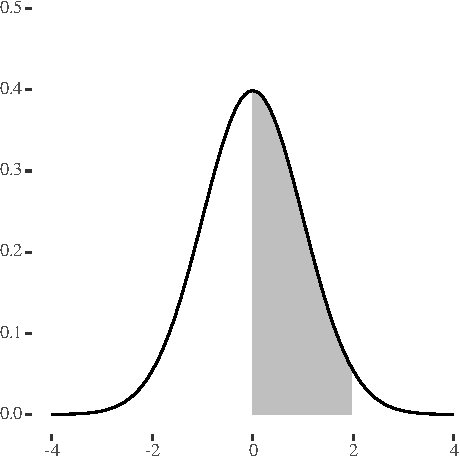
\includegraphics[width=0.8\linewidth]{StandardDivision_files/figure-latex/unnamed-chunk-1-1} 

}

\caption[母標準偏差=1の場合の標本標準偏差の分布]{母標準偏差=1の場合の標本標準偏差の分布}\label{fig:unnamed-chunk-1}
\end{figure}

母集団の標準偏差(\(\sigma\))を変えると分布がどのように変化するか確認する。

\begin{figure}

{\centering \subfloat[母標準偏差=3\label{fig:unnamed-chunk-2-1}]{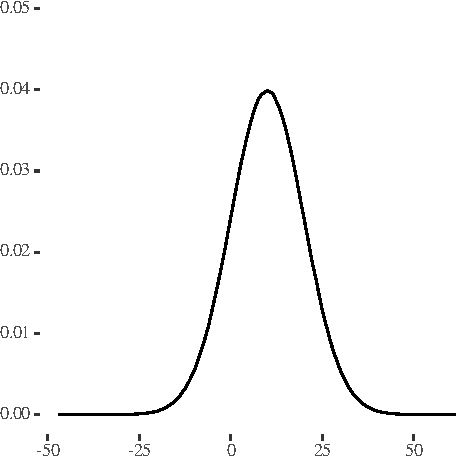
\includegraphics[width=0.4\linewidth]{StandardDivision_files/figure-latex/unnamed-chunk-2-1} }\subfloat[母標準偏差=5\label{fig:unnamed-chunk-2-2}]{\includegraphics[width=0.4\linewidth]{StandardDivision_files/figure-latex/unnamed-chunk-2-2} }

}

\caption[母標準偏差の異なる場合の標本標準偏差の分布]{母標準偏差の異なる場合の標本標準偏差の分布}\label{fig:unnamed-chunk-2}
\end{figure}

母標準偏差(\(\sigma\))が大きくなると右側に裾野が広がっていくことがわかります。

\newpage

\hypertarget{ux504fux5deeux5e73ux65b9ux548cux306eux5206ux5e03}{%
\section{偏差平方和の分布}\label{ux504fux5deeux5e73ux65b9ux548cux306eux5206ux5e03}}

 次に偏差平方和\footnote{\(S = \sum_{i = 1}^{n}{(x_i - \bar{x})^2}\)}の分布をプロットします。偏差平方和は数式を見て分かるように標本標準偏差\footnote{\(s = \sqrt{\frac{\sum_{i = 1}^{n}{(x_i - \bar{x})^2}}{n}}\)}と比例関係にありますので、分布形状も比例するはずです。

\begin{figure}

{\centering 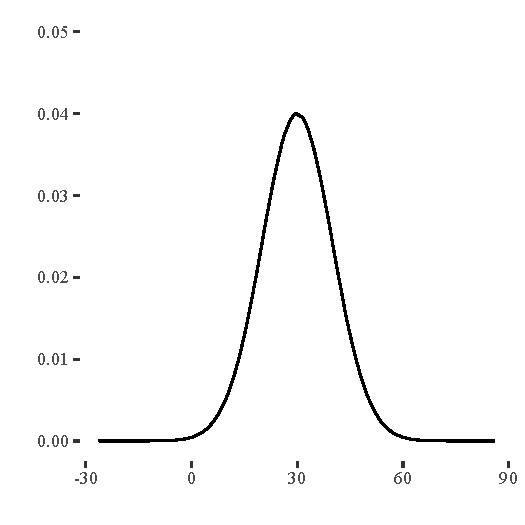
\includegraphics[width=0.8\linewidth]{StandardDivision_files/figure-latex/unnamed-chunk-3-1} 

}

\caption[偏差平方和の分布]{偏差平方和の分布}\label{fig:unnamed-chunk-3}
\end{figure}

\hypertarget{chi2ux5206ux5e03}{%
\section{\texorpdfstring{\(\chi^2\)分布}{\textbackslash chi\^{}2分布}}\label{chi2ux5206ux5e03}}

 \(\chi^2\)分布は下式で定義される分布です。  
\[\chi^2 = \frac{S}{\sigma^2} = \frac{\sum_{i = 1}^{n}{(x_i - \bar{x})^2}}{\sigma^2}\]

\bibliography{bib/references.bib}



\end{document}
